\chapter{Analysis}

\section{Calibration of the parameters}

Having a lot of parameters to calibrate, we decided to limit the number of possible values for each parameter. This choice was made to reduce the number of simulations to be performed and to have a more manageable number of results to analyze. The parameters that we decided to calibrate are the following:

\begin{itemize}
    \item \texttt{meanGenerationTime}: \{20ms, 50ms\} \\
    The mean for the generation times of the processes was chosen by considering a system under heavy and medium load.
    \item \texttt{meanProcessDuration}: \{40ms, 100ms, 200ms\} \\
    The mean for the duration of the processes was chosen after the estimations on the system stability. These values permit to have some combination of parameters that lead to a stable system and others that lead to an unstable system.
    \item \texttt{pCpuBound}: \{0.25, 0.75\} \\
    The probability of a process being CPU-bound has two values, one for a system with a high number of I-O bound processes and the other for a system with a high number of CPU-bound processes.
    \item \texttt{numCpus}: \{1, 4, 12\} \\
    The number of CPUs was chosen to simulate single-core, quad-core, and newer systems with 12 cores.
    \item \texttt{isFCFS}: \{true, false\} \\
    The scheduling policy that the scheduler uses can be either First-Come-First-Served or Shortest-Job-First.
    \item \texttt{generationType}: \{"exponential", "uniform"\} \\
    In addition to the exponential distribution, we also considered the uniform distribution for the generation of processes.
    \item \texttt{durationType}: \{"exponential", "uniform"\} \\
    In addition to the exponential distribution, we also considered the uniform distribution for the duration of the processes.
\end{itemize}


\section{Time parameters setup}

\subsection{Warm-up period}

To determine the warm-up period, we observed the development of the mean number of busy CPUs over time, through 10 independent runs and with different parameters configurations. The number of busy CPUs is a good indicator of the system's stability, as it doesn't depend on the scheduling policy.
Our observations showed that the system stabilizes well before \SI{200}{\second} in all tested configurations. To handle variability and ensure robustness in worse cases, we set the warm-up period to \SI{200}{\second}.

\begin{figure}[H]
    \captionsetup{type=figure}
    \centering
    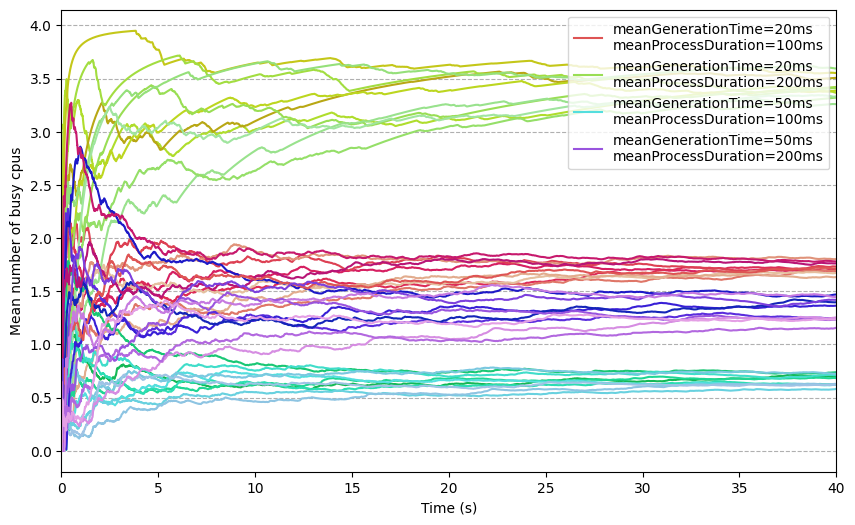
\includegraphics[width=0.9\textwidth]{./images/04/lineWarmup.png}
    \captionof{figure}{Line chart of the mean number of busy CPUs over time for different configurations of meanGenerationTime and meanProcessDuration and multiple repetitions.}
    \label{fig:lineWarmup}
\end{figure}

\begin{figure}[H]
    \captionsetup{type=figure}
    \centering
    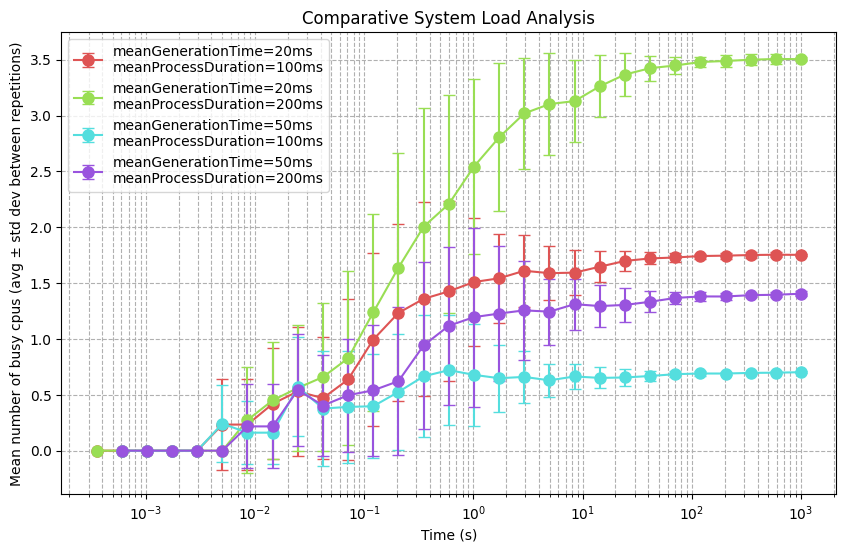
\includegraphics[width=0.9\textwidth]{./images/04/errorWarmup.png}
    \captionof{figure}{Average and Std dev of the mean number of busy CPUs over the repetitions.}
    \label{fig:errorWarmup}
\end{figure}


\begin{table}[H]
\centering
\begin{tabular}{c|cc|cc|cc|cc}
 & \multicolumn{2}{c|}{20ms, 100ms} & \multicolumn{2}{c|}{20ms, 200ms} & \multicolumn{2}{c|}{50ms, 100ms} & \multicolumn{2}{c}{50ms, 200ms} \\
 Time (s) & Avg & Std Dev & Avg & Std Dev & Avg & Std Dev & Avg & Std Dev \\
\midrule
1 & 1.52 & 0.58 & 2.54 & 0.78 & 0.68 & 0.46 & 1.20 & 0.80 \\
2 & 1.54 & 0.37 & 2.85 & 0.64 & 0.67 & 0.27 & 1.25 & 0.51 \\
5 & 1.59 & 0.24 & 3.10 & 0.46 & 0.63 & 0.15 & 1.24 & 0.29 \\
10 & 1.63 & 0.18 & 3.18 & 0.34 & 0.65 & 0.10 & 1.29 & 0.20 \\
20 & 1.68 & 0.11 & 3.33 & 0.22 & 0.64 & 0.08 & 1.27 & 0.15 \\
50 & 1.72 & 0.05 & 3.43 & 0.10 & 0.68 & 0.05 & 1.35 & 0.09 \\
100 & 1.74 & 0.02 & 3.47 & 0.05 & 0.69 & 0.02 & 1.37 & 0.04 \\
200 & 1.75 & 0.02 & 3.49 & 0.05 & 0.69 & 0.02 & 1.38 & 0.03 \\
500 & 1.75 & 0.03 & 3.50 & 0.05 & 0.70 & 0.01 & 1.40 & 0.02 \\
1000 & 1.75 & 0.01 & 3.51 & 0.02 & 0.70 & 0.01 & 1.41 & 0.02 \\
\end{tabular}
\caption{Average and Std dev of the mean number of busy CPUs over the repetitions.}
\label{tab:stabilization}
\end{table}

\subsection{Simulation duration}

For the simulation duration, we chose to end it at \SI{1000}{\second}. This ensures that after discarding the initial \SI{200}{\second} warm-up period, there remains \SI{800}{\second} of simulation data for analysis. Given that the mean generation time is on the order of tenths of seconds, this duration strikes a balance between obtaining statistically meaningful results even after subsampling and maintaining reasonable simulation times.


\subsection{Subsampling}

To analyze the data, the assumption of IID-ness will be needed, but without further modification the samples do not uphold it. For instance, if a process finishes with a large turnaround time, which is caused by a long queue, it is likely that the same thing will happen for the next processes.
To address this and ensure independence between samples, subsampling has been employed. The new sample is constructed taking each point of the starting sample with probability $p$. $p = \frac{1}{2^k}$ and $k$ is the smallest integer that makes $|R(j)| < z_{\alpha/2}/\sqrt{n}$ for each $j$ between 1 and 10.  
This method for choosing k was chosen since only nearby points are correlated.
Before trying a bigger $k$ the condition is tested multiple times with different seeds, this makes sure that $p$ doesn't become too small due to unlucky sampling.
The closer the system is to saturation, the stronger the correlation becomes. As a result, the needed $k$ will become larger, leading to a smaller subsample size.

% todo dare nomi ai grafici con metrica che ti dice quanto saturo (bello se definita nella parte iniziale)

\begin{figure}[H]
    \captionsetup{type=figure}
    \centering
    \begin{subfigure}[b]{0.45\textwidth}
        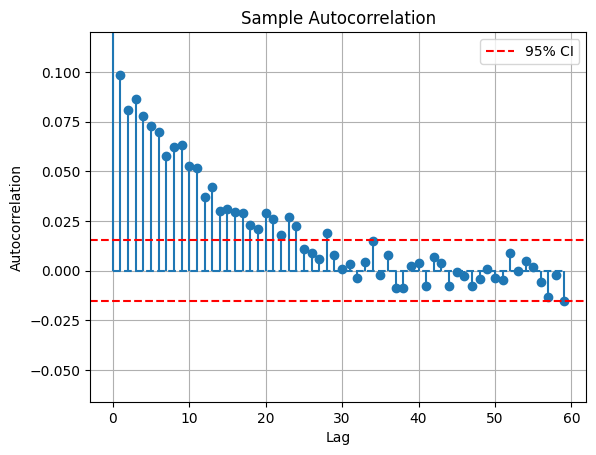
\includegraphics[width=\textwidth]{./images/04/autoCorHighUnfix.png}
        \caption{System close to saturation.}
        \label{fig:autoCorHighUnfix}
    \end{subfigure}
    \hfill % Add space between the subfigures
    \begin{subfigure}[b]{0.45\textwidth}
        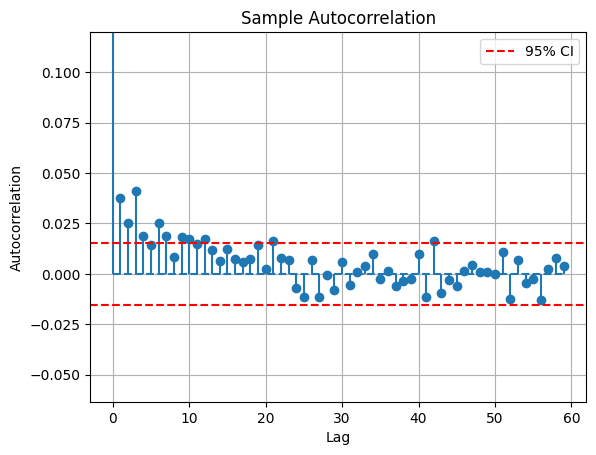
\includegraphics[width=\textwidth]{./images/04/autoCorLowUnfix.png}
        \caption{System with high load but not as close to saturation.}
        \label{fig:autoCorLowUnfix}
    \end{subfigure}
    \vspace{10pt}
    \caption{Comparison of autocorrelation without subsampling for different loads.}
    \label{fig:autoCorComparisonUnfix}
\end{figure}

\vspace{10pt}


\begin{figure}[H]
    \captionsetup{type=figure}
    \centering
    \begin{subfigure}[b]{0.45\textwidth}
        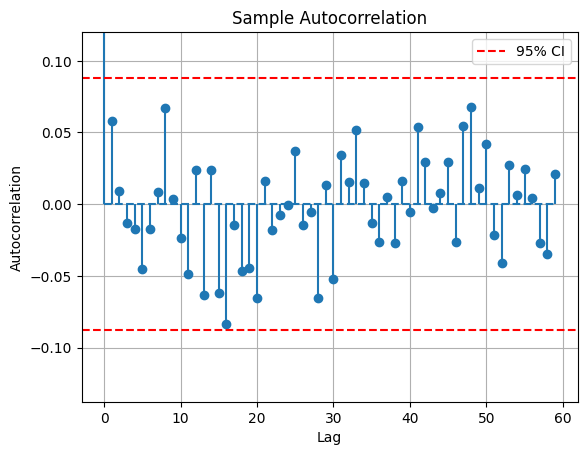
\includegraphics[width=\textwidth]{./images/04/autoCorHighFix.png}
        \caption{System close to saturation with $p=1/32$.}
        \label{fig:autoCorHighFix}
    \end{subfigure}
    \hfill % Add space between the subfigures
    \begin{subfigure}[b]{0.45\textwidth}
        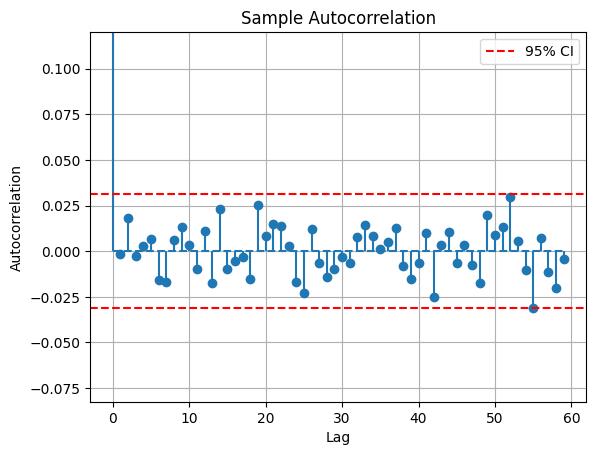
\includegraphics[width=\textwidth]{./images/04/autoCorLowFix.png}
        \caption{System with high load but not as close to saturation with $p=1/8$.}
        \label{fig:autoCorLowFix}
    \end{subfigure}
    \vspace{10pt}
    \caption{Comparison of autocorrelation with subsampling for different loads.}
    \label{fig:autoCorComparisonFix}
\end{figure}